%	Auteur: Surdez Quentin
%	Titre:	 Étudiant MCT
%	Date: Mai 2022
%	Sujet: Rapport de projet P2213	
%============================================================
\documentclass[
	a4paper,									% paper format
	11pt,										% fontsize
	twoside,									% double-sided
	openright,									% begin new chapter on right side
	notitlepage,									% use no standard title page
	parskip=half,								% set paragraph skip to half of a line
]{scrreprt}										% KOMA-script report
%---------------------------------------------------------------------------

\raggedbottom
\KOMAoptions{cleardoublepage=plain}						%Add header and footer on blank pages

%Load Standard Packages: 
%---------------------------------------------------------------------------
\usepackage[standard-baselineskips]{cmbright}				%Fonts for math equation
\usepackage[french]{babel}							%French hyphenation
	%\usepackage[latin1]{inputenc}  					% Unix/Linux - load extended character set (ISO 8859-1)
	%\usepackage[applemac]{inputenc}
	%\usepackage[ansinew]{inputenc}  					% Windows - load extended character set (ISO 8859-1)
%\usepackage[utf8]{inputenc}							%Translate input in latex language
\usepackage[T1]{fontenc}							%Allow a good hyphenation with accentuated language
%\usepackage{tgbonum}
\usepackage{ae}									%Allow vectorial letters
\usepackage{lmodern}
\usepackage{fancyhdr}								%Allow manipulation on headers and tops
\usepackage{graphicx}								%Integration of images
\usepackage{float}									%Better integration of floating objects(tables, etc)
\usepackage{caption}								%For captions of figures and tables
\usepackage{booktabs}								%Nicer tables
\usepackage{tocvsec2}								%Means of controlling the sectional numbering
\usepackage{verbatim}								%Integration of source code
\usepackage{moreverb}								%Extension of verbatim
\usepackage{listings}								%Integration of code in LATEX 
\usepackage{multirow}								%Tables with multiple rows
\usepackage{pdfpages}						
\usepackage{pst-all}								%Better handling of texts and images
\usepackage{mathrsfs}
\usepackage{colortbl}
\usepackage{listings}
\usepackage{minted}
\usepackage{ragged2e}
\captionsetup{font=small}



\newcolumntype{R}[1]{>{\raggedleft\arraybackslash }b{#1}}
\newcolumntype{L}[1]{>{\raggedright\arraybackslash }b{#1}}
\newcolumntype{C}[1]{>{\centering\arraybackslash }b{#1}}		%Adding new column types

%---------------------------------------------------------------------------

%Load Math packages
%---------------------------------------------------------------------------
\usepackage{amsmath}                    				   	% various features to facilitate writing math formulas
\usepackage{amsthm}                       	 				% enhanced version of latex's newtheorem
\usepackage{amsfonts}                      					% set of miscellaneous TeX fonts that augment the standard CM
										
\usepackage{amssymb}							% mathematical special characters
\usepackage{exscale}							% mathematical size corresponds to textsize
\usepackage{listings}
\usepackage{tikz,pgfplots}
\usepackage{array}
%---------------------------------------------------------------------------

%QR Code
%---------------------------------------------------------------------------
\usepackage{qrcode}
\usepackage{subcaption}							%Add sub-caption easily
%---------------------------------------------------------------------------

% Package to facilitate placement of boxes at absolute positions
%---------------------------------------------------------------------------
%\usepackage[absolute]{textpos}
\usepackage[absolute,overlay]{textpos}
\setlength{\TPHorizModule}{1mm}
\setlength{\TPVertModule}{1mm}
%---------------------------------------------------------------------------	

% Definition of Colors
%---------------------------------------------------------------------------
\RequirePackage{color}							% Color (not xcolor!)
\definecolor{linkblue}{rgb}{0,0,0.8}            				% Standard
\definecolor{darkblue}{rgb}{0,0.08,0.45} 				% Dark blue
\definecolor{brickred}{cmyk}{0,0.89,0.94,0.28} 			% Brickred
\definecolor{linkcolor}{rgb}{0,0,0}        					% Black for the print-version!
\definecolor{PEjaune}{rgb}{1,0.84,0}        				% Jaune PE
\definecolor{PEvert}{rgb}{0.14,0.5,0}        				% Vert PE

\definecolor{VertVAUD}{rgb}{0.054, 0.662, 0.301} %14, 169, 77}

%---------------------------------------------------------------------------

% Hyperref Package (Create links in a pdf)
%---------------------------------------------------------------------------
\usepackage[
	pdftex,frenchb,bookmarks,plainpages=false,pdfpagelabels,
	backref = {false},							% No index backreference
	colorlinks = {true},							% Color links in a PDF
	hypertexnames = {true},						% no failures "same page(i)"
	bookmarksopen = {true},						% opens the bar on the left side
	bookmarksopenlevel = {0},					% depth of opened bookmarks
	pdftitle = {Rapport Projet P2213},		   		% PDF-property
	pdfauthor = {Surdez Quentin},        				% PDF-property
	pdfsubject = {Promotion 21-22},        				% PDF-property
	linkcolor = {linkcolor},              					% Color of Links
	citecolor = {linkcolor},              					% Color of Cite-Links
	urlcolor = {linkcolor},               					% Color of URLs
]{hyperref}
%---------------------------------------------------------------------------

% Set up page dimension
%---------------------------------------------------------------------------
\usepackage[
	a4paper,
	left=28mm,
	right=15mm,
	top=30mm,
	headheight=20mm,
	headsep=10mm,
	textheight=242mm,
	footskip=15mm
]{geometry}
\setlength\parindent{20pt}
%---------------------------------------------------------------------------

% Makeindex Package
%---------------------------------------------------------------------------
\usepackage{makeidx}                         					% To produce index
\makeindex                                    					% Index-Initialisation
%---------------------------------------------------------------------------

% Intro:
\pgfplotsset{compat=1.18} 
%---------------------------------------------------------------------------
\begin{document}                              					% Start Document
\settocdepth{subsection}									% Set depth of toc
\pagenumbering{Roman}														
%---------------------------------------------------------------------------

%Set up header and footer
%---------------------------------------------------------------------------
\fancyhf{}												%clean all fields
\fancypagestyle{plain}{									%new definition of plain style
	\fancyfoot[OR, EL]{\footnotesize \thepage}			%footer right part --> page number
	\fancyfoot[OL, ER]{\footnotesize \leftmark}			%footer left part --> chapter
	\fancyfoot[CE, CO]{P2213, QS \& RD}
	\fancyhead[C]{
	\begin{textblock}{0}[0, 0](5, 8)						%header center part --> logo CPNV + MCT 
		
\includegraphics[scale=.7]{img/logoCPNV.png}
	\end{textblock}
	\begin{textblock}{0}[0, 0](175, 3)
		\includegraphics[scale=.5]{img/logoMCT.jpg}
	\end{textblock}
	}
}

\renewcommand{\chaptermark}[1]{\markboth{\thechapter.  #1}{}}
\renewcommand{\headrulewidth}{0pt}				% no header stripline
\renewcommand{\footrulewidth}{0pt} 				% no bottom stripline
\renewcommand\listoflistingscaption{Liste des codes sources}


\pagestyle{plain}
\let\cleardoublepage\clearpage
%---------------------------------------------------------------------------

%=============================================================================================
% Page principale
%=============================================================================================
%---------------------------------------------------------------------------
\begin{titlepage}
	\setlength{\unitlength}{1mm}
%	\begin{textblock}{230}(-10,-10)
%		\begin{picture}(230,35)%32)
%			\put(73,0){\color{VertVAUD}\rule{160mm}{40mm}}
%		\end{picture}
%	\end{textblock}

	\begin{textblock}{0}[0,0](5,12) % (x,y)
		
\includegraphics[scale=1]{img/logoCPNV.png}
	\end{textblock}

	\begin{textblock}{0}(158, 4)
		\includegraphics[scale=.7]{img/logoMCT.jpg}
	\end{textblock}





% Titre / Sous-titre / Auteur / Image de garde:
%---------------------------------------------------------------------------
	
	\flushleft
	\vspace*{1cm}
	%\fontfamily{cmr}\selectfont			%To have the default font
	\fontsize{18pt}{20pt}\selectfont
	CPNV - Centre Professionnel du Nord Vaudois \\
	\fontsize{12pt}{15pt}\selectfont\vspace{0.5em}
	MCT - Modules complémentaires techniqeus

	\vspace{3cm}

	\fontsize{30pt}{32pt}\selectfont 
	\noindent \textbf{Explication code Arduino} \\

	\fontsize{18pt}{20pt}\selectfont\vspace{0.3em} P2213 \\

	\vspace{4cm}
	\fontsize{12pt}{15pt}\selectfont
	\begin{tabbing}
		xxxxxxxxxxxxxxx\=xxxxxxxxxxxxxxxxxxxxxxx \kill
		Rédacteur:\> Quentin Surdez\\ \\
		Relecture:\> Rafael Dousse\\ \\
		École:\> CPNV\\ \\
		Date:\> Yverdon-Les-Bains, le \today \\
	\end{tabbing}
\end{titlepage}
%---------------------------------------------------------------------------

%===========================================
% Table des matières
%===========================================
\tableofcontents

\listoffigures									% Table des figures
%\listoftables									% Table des tableaux
%\listoflistings % Now typeset the list
\cleardoublepage
%---------------------------------------------------------------------------

%=============================================================================================
% Introduction
%=============================================================================================
\pagenumbering{arabic}
\setcounter{page}{1}

\chapter{Introduction}
Ce document a pour but d'expliciter les commentaires et l'architecture du code de l'Arduino Nano pour le contrôle des moteurs. Il permet un approfondissement du code et de comprendre la logique derrière 
les différents choix effectués.

%=============================================================================================
% Document
%=============================================================================================

\chapter{Asservissement des moteurs}

L'asservissement de moteurs à courant continu est au coeur de notre projet. En effet, chaque fonction que nous construisons par la suite reposera totalement ou en partie sur la fonction d'asservissement. \par

L'asservissement permet de contrôler un certain paramètre dans un système. Il se caractérise par le besoin d'un système de maintenir une consigne donnée, qu'importe les perturbations infligées au système.
Nous avons donc asservi notre système au niveau des moteurs. En effet, nous souhaitons que le robot aille tout droit lorsqu'on le lui demande, ce qui se traduit par le besoin d'avoir
la même vitesse constante aux deux moteurs. \par

\section{PID}



Pour asservir nos moteurs à courant continu, nous avons choisi d'utiliser la méthode des facteurs PID. L'acronyme PID signifie proportionnel, intégral, dérivateur. Ce sont les 3 facteurs que nous 
utilisons pour construire notre asservissement. \par

Pour utiliser les différents facteurs, nous devons premièrement calculer l'erreur. Elle est la différence entre la consigne et la vitesse observée. Nous appliquons le facteur proportionnel directement à l'erreur.
Le facteur intégratif est appliqué à la somme des erreurs sur le temps. Enfin, le facteur dérivateur s'applique sur la différence des erreurs sur le temps. \par



L'équation pour le calcul de la valeur de contrôle est la suivante : 
		\begin{figure}[h]
			\[u=k_pe + k_i \int e \cdot dt + k_d \cfrac{de}{dt}\] 
			\caption{Équation du PID}
			\label{eq1}
		\end{figure}


Les différents calculs se font par rapport à un $dt$, cette particularité est très importante et a permis de diriger le développement du code. Pour mieux comprendre l'intégration de l'équation dans le code 
une image permet de visualiser le processus : 

	\begin{figure}[h!]
		\centering
		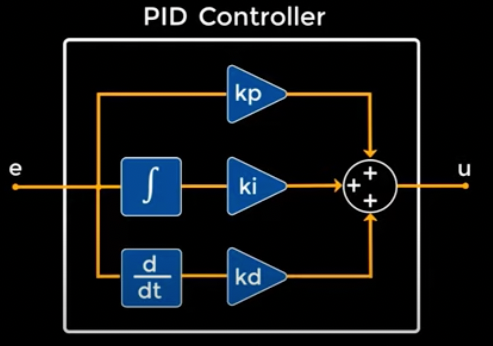
\includegraphics[scale=.3]{img/PID.png}
		\label{PIDfig}
		\caption{Intégration de l'erreur et du PID}
	\end{figure}
\par


\chapter{Interruptions}

Comme expliqué au-dessus, la composante du temps est très importante. C'est grâce à elle que l'asservissement peut être fonctionnel et robuste. Pour intégrer ce besoin, il existe une fonctionnalité 
des microcontrôleurs MegaAVR appelée interruption. Les interruptions permettent, comme leur nom l'indique, d'interrompre le programme pour effectuer une tâche bien précise. Souvent, cette tâche est une incrémentation de valeur, ainsi 
l'interruption ne dure qu'un très court instant. Après avoir fini la routine d'interruption, le programme reprend exactement là où il en était. \par

\section{Les interruptions attachées}

La librairie Arduino permet d'utiliser une fonction appelée attachInterrupt(). Cette fonction permet de donner à un pin la responsabilité de lancer une routine d'interruption. Cette interruption sera alors attachée à un pin. Ainsi, si un pin est activé 
à un internal de temps régulier, la routine d'interruption se fera à un interval de temps régulier. \par

Cela a été mis en place pour notre projet en incorporant un Arduino gérant exclusivement le temps. Toutes les $x$ secondes, un signal est envoyé à l'Arduino se chargeant de calculer le PID. Un schéma permet de visualier 
le processus : 
\par

\begin{figure}
	\centering
	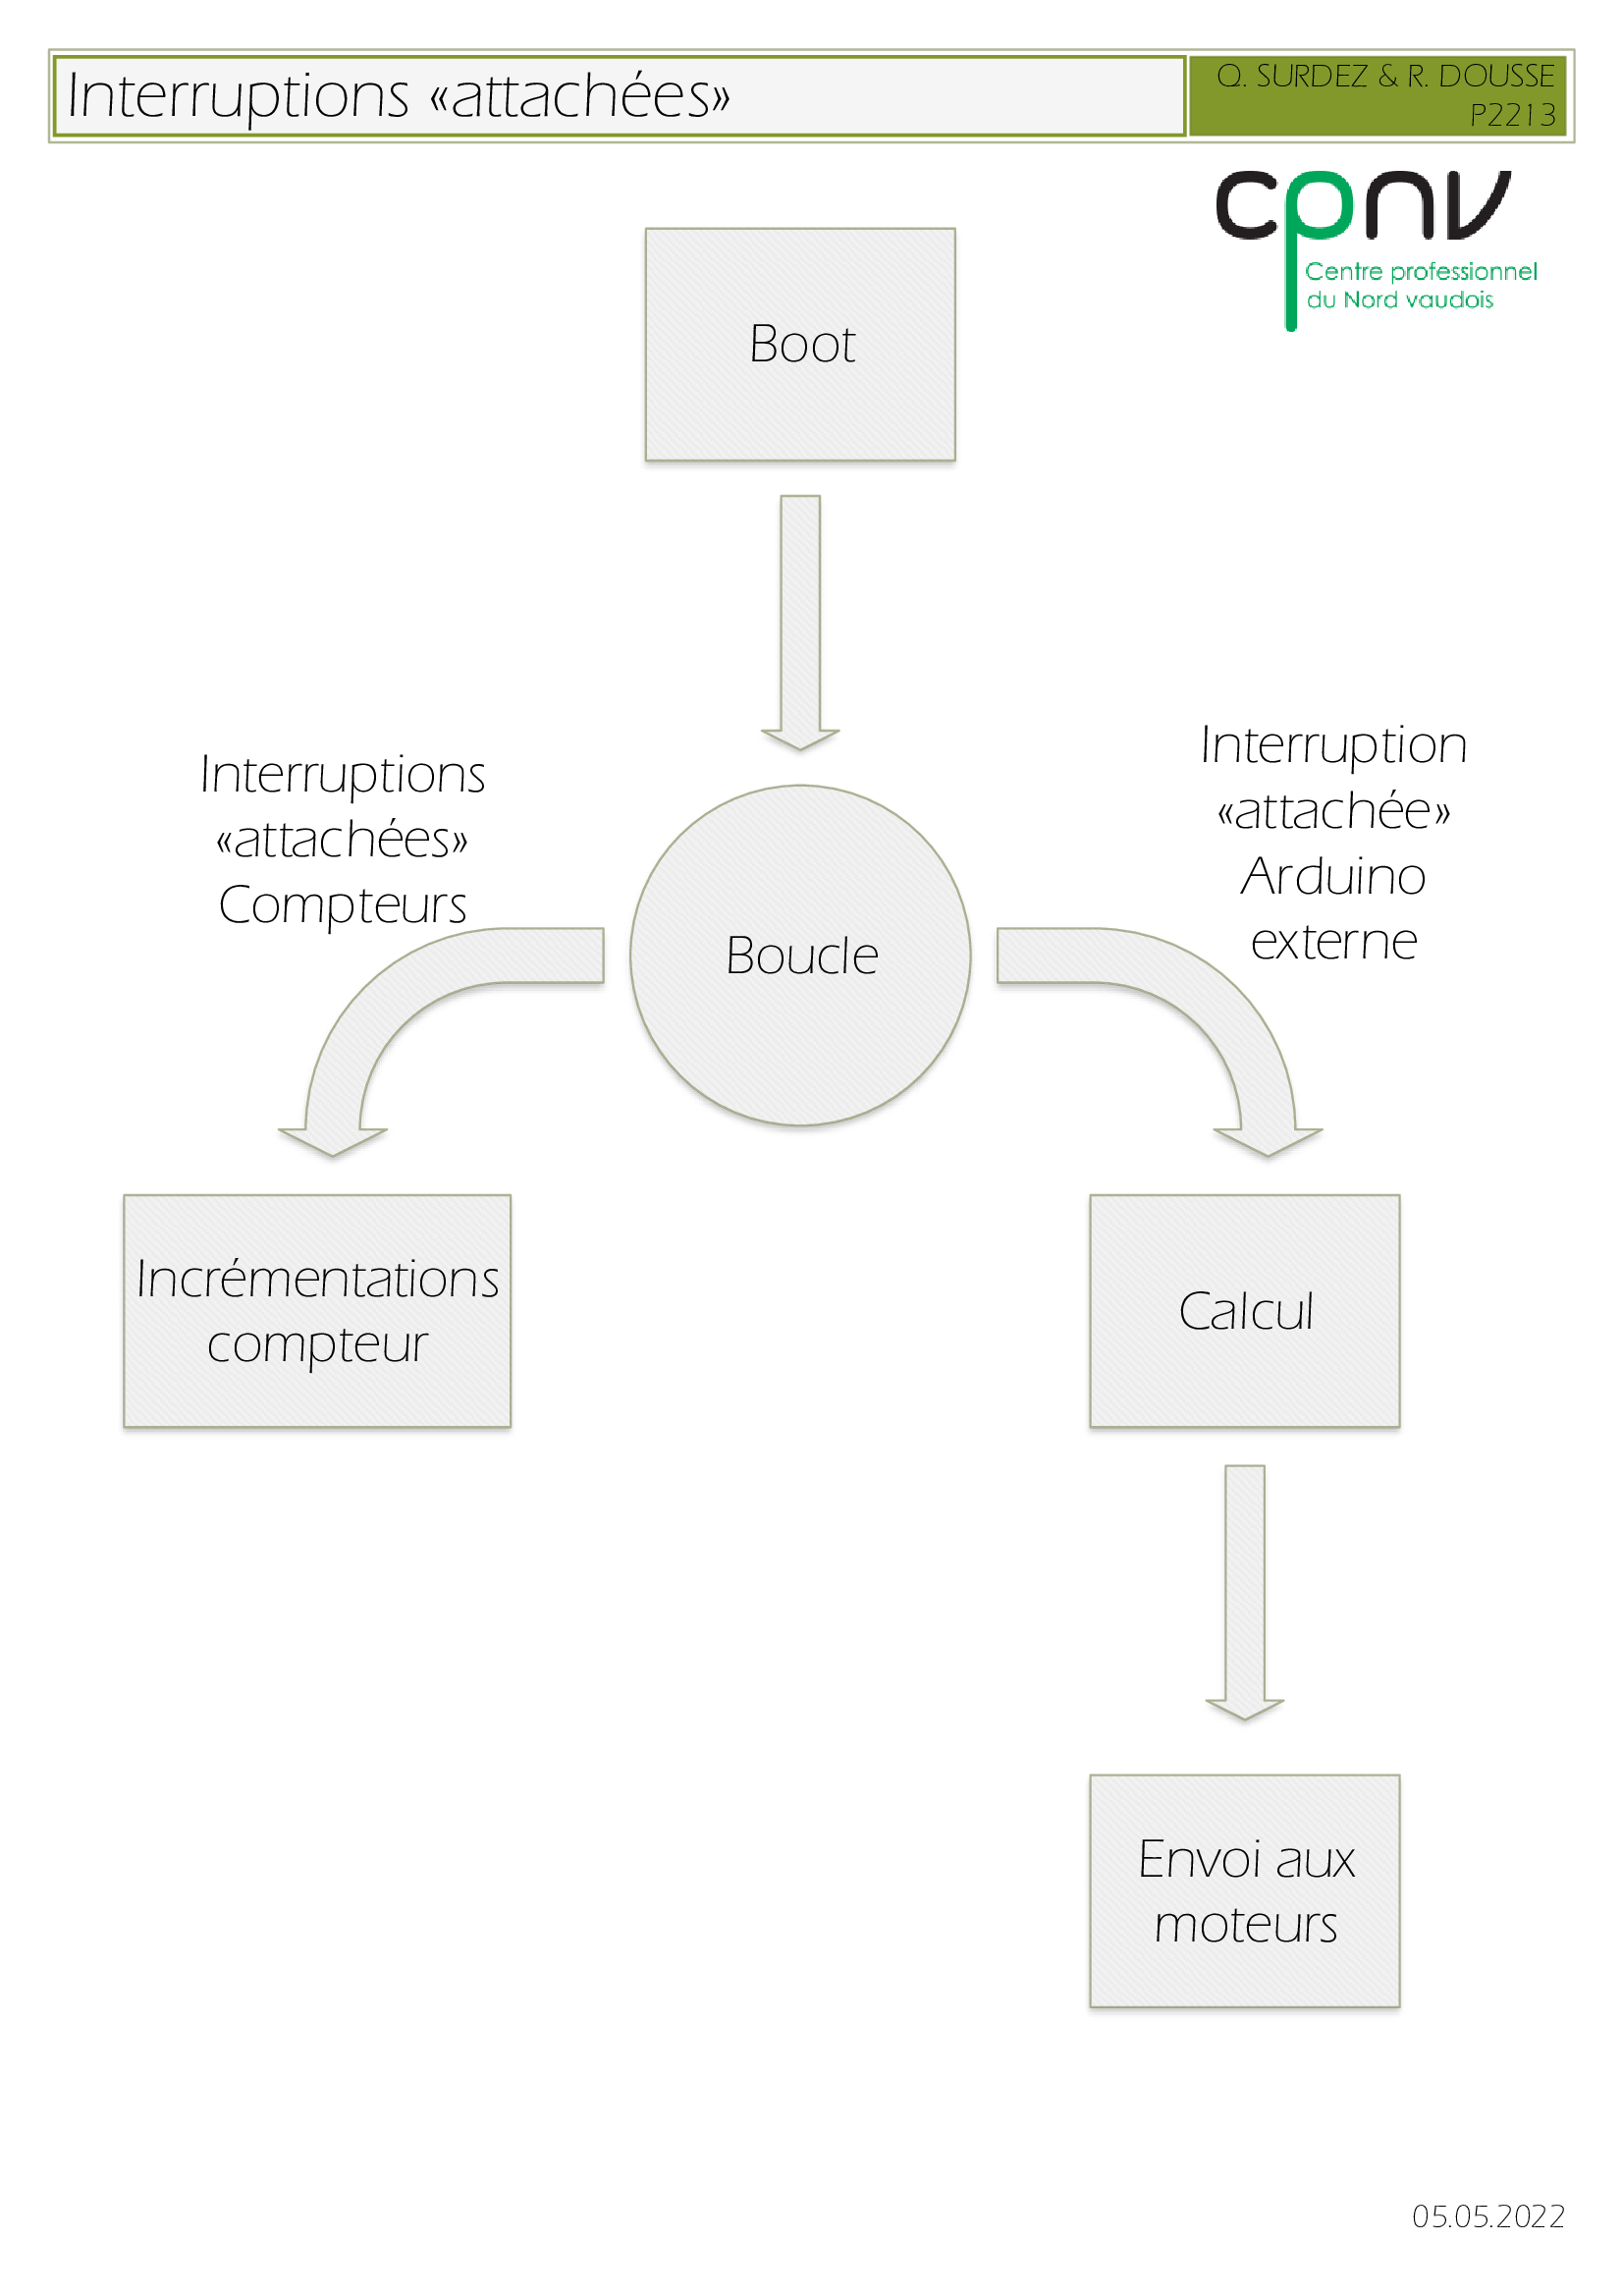
\includegraphics[scale=0.2]{img/interruptions_attachees.jpg}
	\label{IntSch}
	\caption{Schéma des interruptions attachées}
	
\end{figure}


\chapter{Code}

Le code a été écrit dans le but de répondre au besoin de notre projet. Les fonctions le composant et la logique appliquée
seront discutés dans les prochains sous-chapitres. Premièrement, une explication du code nécessaire au setup de la
communication I2C, puis donner de plus grandes explications que les commentaires sur les fonctions créées. Enfin, une
une explication sur la remise à zéro des différentes valeurs pour que les différentes fonctions puissent intéragir entre
elles sans compromettre l'intégrité de l'ensemble.

\section{Communication I2C}

La communication I2C est celle que nous utilisons dans le cadre de notre projet. Ce mode de communication est rapide (moins d'une seconde) et permet de rajouter des slaves facilement
dépandamment de nos besoins. La librairie Wire.h avec Arduino permet une mise en place simple des différentes fonctions utilisées. \par

Pour commencer, son setup est composé de deux fonctions. La première est celle déterminant l'adresse donnée au microcontrôleur slave et la deuxième est celle qui détermine quelle
fonction appelée lorsque le slave reçoit un ordre du master. Les voici : 
\begin{figure}[!ht]
	\usemintedstyle{rainbow_dash}
	\begin{minted}{c}
// Set up de la communication avec le Raspberry PI via I2C -----------------
Wire.begin(0x08);
Wire.onReceive(receiveEvent);
	\end{minted}
	\caption{Setup I2C}
	\label{codeI2C}
	\end{figure}

Nous pouvons voir que nous choisissons l'adresse 08 et qu'une fonction (receiveEvent) est appelée à chaque
fois que l'Arduino reçoit une information de la part du maître soit le Raspberry PI dans notre cas. 

\newpage
\section{Fonctions appelées}

La première fonction appelée lors de la réception d'un ordre est donc, comme vu ci-dessus, receiveEvent(). 
Voici sa structure : 

\begin{figure}[!ht]
	
	\usemintedstyle{rainbow_dash}
	\begin{minted}{c}
// Communication avec le Raspberry via I2C --------------
void receiveEvent(int howMany){
  while(Wire.available()){
    int c = Wire.read();
    switch (c)
    {
    case 3:
      cinqMenAvant();
    break;
    case 4:
      tourneSurSoi();
    break;
    case 10:
      toutDroit();
    break;
    }
  }
}
	\end{minted}
	\caption{Fonction de réception et de commande}
	\label{receiveEvent}
	\end{figure}

Nous pouvons voir que la fonction vérifie en premier lieu que le bus I2C est libre. Ensuite on stock la valeur 
qu'on lit sur le bus dans une variable locale. Cette dernière, dépendamment de sa valeur permet d'enclencher 
une fonction ou une autre. Nous utilisons un switch pour choisir la fonction. Nous avons ici trois cas :

\begin{itemize}
	\item cinqMenAvant(), la fonction qui permet au robot d'aller tout droit pendant 5$m$, puis de s'arrêter
 	\item tourneSurSoi(), la fonction qui permet au robot de faire un tour sur lui-même, puis de s'arrêter
  	\item toutDroit(), le robot se met en marche avec le PID et ne s'arrête pas
\end{itemize}

\noindent Nous allons observer la structure commune de ces fonctions avec cinqMenAvant() : 
\newpage
\begin{figure}[!ht]
	
	\usemintedstyle{rainbow_dash}
	\begin{minted}{c}
// Set up du programme 5m en avant --------------------------------------
void cinqMenAvant(){
  
  tick_distance=0;
  tick_distance1=0;
  enAvant = 1;

  //Interruptions 
  attachInterrupt(digitalPinToInterrupt(photoElectricSensor), compteurDistance, RISING);
  attachInterrupt(digitalPinToInterrupt(photoElectricSensor1), compteurDistance1, RISING);
  attachInterrupt(digitalPinToInterrupt(pin_PID), asservissement, RISING);

  //On donne une consigne petite pour être sûr que le robot va tout droit
  consigne_moteur = 2;
  consigne_moteur1  = 2;
}
	\end{minted}
	\caption{Fonction pour se déplacer 5m en avant}
	\label{cinqMenAvant}
	\end{figure}
Nous pouvons voir ci-dessus que les premières variables que nous changeons sont celles qui sont inhérentes
à la fonction. Les $tick\_distance$ permettent de s'assurer qu'ils soient à zéro au lancement. Ce sont eux qui gèreront
la distance parcourue. Ensuite, la variable $enAvant$ sera approfondie dans le prochain chapitre. \par

Nous voyons enfin ce qui nous intéresse particulièrement, les interruptions attachées. Elles sont à gérer pour
chaque appel de fonction. Le setup des interruptions se fait exculsivement à ce moment précis. Nous choisissons 
les pins liés aux interruptions, quelle fonction la routine appelera et le mode sur lequel la routine se déclenchera. 
Ensuite, les consignes moteurs sont définies pour le calcul du PID. \par

Les différentes fonctions utilisées, ont toutes la même strucutre avec de léger changement comme la consigne moteur qui
est à 0 sur un moteur pour que le robot tourne sur lui-même. Cependant, si un clean up n'est pas correctement effectué 
avant l'appel d'une autre fonction, les interruptions ne se comporteront pas de la bonne manière. Ainsi, il 
faut remettre les différentes valeurs à zéro. 

\section{Remise à zéro des valeurs}

La remise à zéro des valeurs s'effectue à la sortie des fonctions, ou plus précisément, lorsque ces dernières 
ont rempli le rôle qui leur était attribué. La limite de ce système est qu'il ne gère pas le cas où 
une fonction n'est pas finie et une autre est appelée. \par

Les variables que nous changeons dans les fonctions comme $enAvant$ nous servent à désattacher les interruptions
lorsque le travail de la fonction est terminée. Cette action se fait dans le loop() de notre script Arduino. \par

\noindent Voici un exemple pour la fonction cinqMenAvant() : 
\newpage
\begin{figure}[!ht]
	
	\usemintedstyle{rainbow_dash}
	\begin{minted}{c}

if (enAvant == 1){
  
  // Limite du nombre d'incrémentations pour que le robot fasse 5m depuis l'allumage
  if (tick_distance >= 580){
	setMotor(1, 0, Enable1, In1, In2);
	setMotor(1, 0, Enable2, In3, In4);
	detachInterrupt(digitalPinToInterrupt(photoElectricSensor));
	detachInterrupt(digitalPinToInterrupt(photoElectricSensor1));
	detachInterrupt(digitalPinToInterrupt(pin_PID));
	Serial.println("5m atteint");
	enAvant= 0;
  }
}
	\end{minted}
	\caption{Clean up de la fonction cinqMenAvant()}
	\label{remise0}
	\end{figure}

 Pour rentrer dans le $if$ principal, il faut que la fonction cinqMenAvant() ait été appelée. Ensuite, nous avons
 la condition qui déclenche le clean up. Au début du clean up, les moteurs sont forcés à 0 par la fonction setMotor(). 
 Ensuite, les interruptions sont détachées. Celle qui permet de calculer le PID est la plus importante pour 
 être certain qu'aucun calcul ne sera effectué. Enfin, une mise à zéro de la variable $enAvant$ permet de sortir 
 du clean up. 

 \chapter{Conclusion}
 Nous avons pu nous intéresser aux différentes composantes du script de notre Arduino Nano Every. Cela permettra au 
 lecteur attentif de gérer et adapter le code écrit selon ses besoins. Le peu de fonctions qui n'ont pas été introduites
 dans le document, possèdent suffisamment de commentaires pour être clair et compréhensible par le lecteur. \par

 Le développement du code se sera fait à travers maintes itérations. La version présentée aujourd'hui est dans 
 sa phase finale. Incorporant la communication avec le Raspberry PI, elle se veut prête à répondre aux 
 besoins du projet. La flexibilité des attachInterrupt() et detachInterrupt() permettent facilement de passer
 d'une fonction à l'autre, aussi longtemps que le clean up est correctement effectué.

\end{document}